\begin{exercise}
      {ID-10e0afc81a3188f6abe80a9c6665b0b8e966960b}
      {Wie viel fehlt hier?}
  \ifproblem\problem\par
    Die folgende Abbildung zeigt die zu untersuchende Figur für $n=7$. Stelle einen Term
    $A(n)$ für die Fläche der Figur auf. Erläutere in einem Satz und durch eine ausführlich
    beschriftete Zeichnung, wie dieser Term zustande kommt.\par
    Berechne $A(7)$, $A(30)$ und $A(101)$.
    \begin{center}
      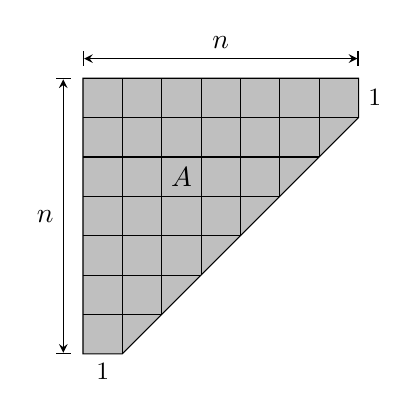
\begin{tikzpicture}[scale=0.5]
        \filldraw[fill=black!25!white] (0, 0) -- (0, 7) -- (7, 7) -- (7, 6) -- (1, 0) -- cycle;
        \begin{scope}
          \clip (0, 0) -- (0, 7) -- (7, 7) -- (7, 6) -- (1, 0) -- cycle;
          \draw (0, 1) -- (7, 1);
          \draw (0, 2) -- (7, 2);
          \draw (0, 3) -- (7, 3);
          \draw (0, 4) -- (7, 4);
          \draw (0, 5) -- (7, 5);
          \draw (0, 6) -- (7, 6);
          \draw (1, 0) -- (1, 7);
          \draw (2, 0) -- (2, 7);
          \draw (3, 0) -- (3, 7);
          \draw (4, 0) -- (4, 7);
          \draw (5, 0) -- (5, 7);
          \draw (6, 0) -- (6, 7);
        \end{scope}
        \begin{scope}[xshift=-5mm]
          \draw[>=stealth, |<->|] (0, 0) -- node[left] {$n$} (0, 7);
        \end{scope}
        \begin{scope}[yshift=5mm]
          \draw[>=stealth, |<->|] (0, 7) -- node[above] {$n$} (7, 7);
        \end{scope}
        \node[right] at (7, 6.5) {\small1};
        \node[below] at (0.5, 0) {\small1};
        \node at (2.5, 4.5) {$A$};
      \end{tikzpicture}
    \end{center}
  \fi
  %\ifoutline\outline\par
  %\fi
  %\ifoutcome\outcome\par
  %\fi
\end{exercise}
